% This file was converted to LaTeX by Writer2LaTeX ver. 1.6
% see http://writer2latex.sourceforge.net for more info
\documentclass[a4paper]{article}
\usepackage[utf8]{inputenc}
\usepackage[noenc]{tipa}
\usepackage{tipx}
\usepackage[geometry,weather,misc,clock]{ifsym}
\usepackage{pifont}
\usepackage{eurosym}
\usepackage{amsmath}
\usepackage{wasysym}
\usepackage{amssymb,amsfonts,textcomp}
\usepackage[T3,T1]{fontenc}
\usepackage[varg]{txfonts}\usepackage[english]{babel}
\usepackage{color}
\usepackage[top=2cm,bottom=2cm,left=2cm,right=2cm,nohead,includefoot,foot=0.986cm,footskip=1.871cm]{geometry}
\usepackage{array}
\usepackage{hhline}
\usepackage{hyperref}
\hypersetup{pdftex, colorlinks=true, linkcolor=blue, citecolor=blue, filecolor=blue, urlcolor=blue, pdftitle=}
\usepackage[pdftex]{graphicx}
% Text styles
\newcommand\textstylest[1]{#1}
\newcommand\textstyleFootnoteAnchor[1]{\textsuperscript{#1}}
% Footnote rule
\setlength{\skip\footins}{0.119cm}
\renewcommand\footnoterule{\vspace*{-0.018cm}\setlength\leftskip{0pt}\setlength\rightskip{0pt plus 1fil}\noindent\textcolor{black}{\rule{0.25\columnwidth}{0.018cm}}\vspace*{0.101cm}}
\title{}
\begin{document}
\section{Philosophy in science: A name with a long intellectual tradition}


\begin{figure}[htp]
\centering
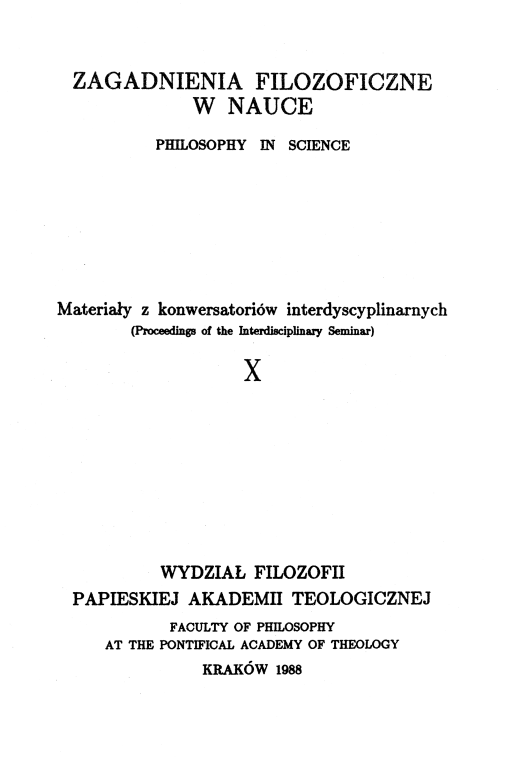
\includegraphics{Polakorg-img001.png}
\end{figure}
The term “philosophy in science” has been in use for at least 40 years. It was first proposed in the late 1970s during
the seminars held in Kraków by the scientists and philosophers working with Michael Heller and Józef Życiński. Over the
years, these seminars evolved into the Center for Interdisciplinary Studies \label{ref:RNDVHajAQnl1F}(see Trombik,
2019), which had its own journal, namely \textit{Zagadnienia Filozoficzne w Nauce}. The term “philosophy in science”
was used to denote the distinctive character of the philosophical topics discussed in his journal. Since the first
issue, in addition to its Polish title \textit{Zagadnienia Filozoficzne w Nauce }(1978/1979), also featured on its
cover page the English equivalent “Philosophy in Science” (see picture).\footnote{The same concept of philosophy was
also applied in a second journal edited by Heller and Życiński (also co-edited by W.R. Stoeger) entitled
\textit{Philosophy in Science}. This journal was also published by the Center for Interdisciplinary Studies (Vatican
Observatory and Pontifical Academy of Theology in Kraków) by the Pachart Publishing House (during 1983–2003). The
periodical \textit{Zagadnienia Filozoficzne w Nauce }was initially published in Polish, while \textit{Philosophy in
Science }was published in English. The current editions of the former periodical are now bi-lingual and cover both the
English and Polish versions. The English title, \textit{Philosophical Problems in Science, }is a direct translation of
the original Polish title \textit{Zagadnienia Filozoficzne w Nauce. }We keep this name because it reveals an important
aspect of this approach, namely a focus on philosophical problems relating to science. The significance of this
difference will become clear after reading this paper.}

One article that defined the concept of “philosophy in science” also became a reference for methodological and
metaphilosophical discussions about the roles of philosophy in science and of science in philosophy, specifically in
Poland. This was Michael Heller’s paper titled \textit{Jak możliwa jest filozofia w nauce?} (\textit{How is Philosophy
in Science Possible}?) \label{ref:RNDrCU7rgcyDR}(Heller, 1986).\footnote{Józef Życiński shared Michael Heller's concept
of philosophy in science, but he focused on different aspects. A good example of this distinction is the co-authored
article in which Życiński takes many parts of Heller's text verbatim and exposes in them new epistemological aspects of
science and philosophy relationships that are not obvious in Heller’s original text \label{ref:RNDzM7nNfibOc}(Heller
and Życiński, 1987).} The impact of this article, despite its historic significance, has been limited because the text
has only been available in Polish. Hopefully this publication of an English translation of Heller’s article, together
with a commentary, will fill this gap.

\subsection{1. The historical context of Heller’s publication}
Heller’s paper needs to be viewed from the historical context. In sixties of the 20\textsuperscript{th} century, Polish
philosophy was entangled in a debate about the concept of the philosophy of science that was later described as
counter-productive. The debate was provoked by Kazimierz Kłósak’s papers about the traditional neo-scholastic
philosophy of nature that were published around this time (Heller, 1995, p.150). Heller considered this debate
misguided, however. In his view a new approach to the philosophy of science was needed that would differ from Kłósak’s
\textit{a priori} method. The new approach also required a name that would differentiate it from older
approaches.\footnote{It is worthwhile noting that Michael Heller used the traditional name of the \textit{philosophy of
nature }(\textit{filozofia przyrody}) in the sense of philosophy in science when it does not lead to misunderstandings,
and he sometimes used this term in the broader sense of the “philosophical theory of nature.” He formulated two
necessary conditions that this “theory of nature” must satisfy: “(a) it cannot be a theory that ignores the natural
sciences in whatever domain it studies, and (b) it cannot ignore at least the fundamental methodological rules
elaborated by the contemporary philosophy of science.” The meaning of these requirements is clarified by the following
remark: “Violations of the first condition make the given philosophical conception an anachronism; neglect of the
second condition threatens methodological anarchy” (Heller, 2011b, p.157).}

Together with Życiński, Heller aimed to create a philosophy grounded in science but harmonized with the Christian faith.
This philosophy was supposed to compete with Kłósak’s traditional philosophy of nature, and it was conceived as a
modern, non-standard interpretation of the \textit{ad mentem St. Thomae }metaphilosophical rule (Leo XIII,
\textit{Aeterni Patris}, 1879). The new philosophy was intended to create a framework for science–religion studies that
accounted for the most modern scientific knowledge. 

In those years, Krakow, with its tradition of interdisciplinary debates, was a special place for engaging in the
philosophy of science. At the center of these disputes was one Karol Wojtyła (Życiński, 1999, p.8nn), who later became
Pope John Paul II . He organized and encouraged seminars and informal discussions among scientists and philosophers.
Philosophical discussions that were initially rather informal continued with great success at more formal
interdisciplinary meetings and seminars. The debates convinced Michael Heller that a new philosophy of science, which
he denoted as “philosophy in science”, was needed, one that should be founded on the assumption that philosophy must
have an interdisciplinary character (Heller and Mączka, 2006, p.50), because it could not exist in isolation from other
scientific disciplines. The second assumption, one inspired by positivist philosophy, was that modern science should
serve as a tool for clarifying or solving classical philosophical problems (Heller and Mączka, 2006, p.50). However,
contrary to positivist philosophy, which perceives classical philosophical problems (e.g., metaphysical issues) as
fully reducible to science, the \textit{philosophy in science }proposed by Heller saw these problems as having their
own nature, one that transcended scientific methods.

\subsection{2. Philosophy in science: A metaphilosophical concept}
“‘Philosophy in science’ grew out of practice” (Heller, 2019, p.ref1): This sentence in the opening paragraph of
Heller’s paper reveals the source of this philosophy. The term “practice” may mean two things. It may denote
philosophical reflection by scientists on their own research (e.g., philosophizing physicists), or it may refer to the
concept of \textit{philosophy in science}, which is a specific mode of philosophical reflection practiced by the
philosophers and scientists in the Kraków milieu. 

The former interpretation shows that the intuitions and the actual praxis both play equally fundamental roles in
\textit{philosophy in science}, and this philosophy should be undertaken with knowledge of hard facts and be
enlightened by intuitions. Heller (2011b, p.86) pointed out that neglecting scientific results and a lack of scientific
intuition led philosophy astray. The former was the source of poverty in the German romantic philosophy of nature,
while the latter led neo-scholastics to a false interpretation of the role of St. Thomas Aquinas’s philosophy. In the
“Introduction” to the \textit{Philosophy in Science }journal, we find the following statement:

\begin{quotation}
\textit{One of the most dangerous movements of traditional philosophy has been its attempt to develop philosophical
analyses independently of scientific results. And one of the most hopeless illusions of
19}\textit{\textsuperscript{th}}\textit{ century science was its desire to replace philosophy by science and to give
scientific answers to questions posed by classical philosophy (Heller, Stoeger and Życiński, 1983, p.7).}

\end{quotation}
Grounding \textit{philosophy in science }in scientific praxis was behind Heller’s aversion to the formalization of
philosophy. Philosophy should take place spontaneously as part of scientific work. One may claim that
\textit{philosophy in science }has in fact been practiced from the very beginning of the history of empirical sciences.
For example, looking at Newton’s work, it is difficult to determine whether it is of a scientific or philosophical
nature, or was it already a form of \textit{philosophy in science }(Heller, 2019, p.ref2)?

For a long time, Heller avoided publishing any formal declarations or manifestos. He preferred to have tangible results
that would speak for themselves (and his philosophy) rather than developing a complete theory. In his view, philosophy
could generally be accurately characterized only \textit{ex post,}\footnote{Michael Heller wrote: “I believe, however,
that the time has come for an attempt to systematize what \textit{de facto} is ‘philosophy in science’” (Heller, 2019,
p.ref8).} and any \textit{a priori }claims about philosophy may be misleading and dangerous. He formulated only one
necessary condition for practicing \textit{philosophy in science}: “I would only protest against calling some
meta-considerations that are not rooted in scientific practice ‘philosophy in science’” (Heller, 2019, p.ref3). This
statement (Heller, 1986) could suggest an approval of a chaotic approach to philosophical work. However, a critical
assessment of the traditional rigid methodology does not imply methodological anarchy or philosophical
\emph{laissez}\textstylest{{}-}\emph{faire}. Anticipating this interpretation, Heller clearly stated that “developing
philosophy in science cannot generate an epistemological chaos” (Heller, Stoeger and Życiński, 1983, p.8). Thus, to
correctly understand Heller’s idea, we need to keep this declaration in mind.

The supremacy of practical science over purely intellectual pursuits as a source of philosophical insight reveals
another facet of Heller’s philosophy, namely its evolutionary character. Heller viewed philosophy as being engaged in
an endless process of adjusting to science. Science is largely not static, so \textit{philosophy in science }also
should not be, because philosophy in science cannot remain blind to what occurs in the sciences. For Heller, the
continuous development of philosophy is possible, because he conceived his philosophy as non-foundational.\footnote{In
Heller’s view, fundationalist philosophy is a philosophy that provides indubitable knowledge, and it is grounded in the
incontestable fundamentals (Heller, 2006b). This kind of fundationalism is called \textit{methodological fundationalism
}by Heller, because it describes a philosophical method. The methodological fundationalism is opposed by psychological
fundationalism, which requires indubitable grounds for knowledge. Anti-fundationalist philosophy rejects incontestable
fundamentals and replaces them with hypothetical claims. This type of philosophy could never create a conceptually
closed (complete) system. However, this philosophy improves philosophical methodology and clarifies conceptual
resources.} His philosophy is consequently minimalistic in the sense that it, as a rule, avoids the creation of a
closed, static, defined, and rigid philosophical system (Heller, 2006a, p.34).

Michael Heller also stressed another metaphilosophical assumption behind \textit{philosophy in science}, namely the
possibility for a dialogue between philosophy and science. This assumption led him to reject the “doctrine of
non-intersecting planes.” The paradigmatic representation of this doctrine was a neo-scholastic philosophy of nature
based on Jacques Maritain’s concept of separation science from philosophy and theology. This principle, even if it
seemed to be more logical or better than the non-separation methodologies, was unable to resolve the conflicts between
science and philosophy precisely because of its \textit{a priori} assumed separation. Thus, because of this\textit{ a
priori} assumption, as well as its heavy historical baggage from its origins in scholastic philosophy, Jacques
Maritain’s approach to philosophy has been generally criticized and rejected by both philosophers of science and
scientists. Scientists, in reaction to the poverty of classical philosophy, attempted to create their own form of
philosophy, one inspired by their own scientific practices using their own scientific methods. Unfortunately, these
philosophies made by scientists for scientists have been frequently judged by philosophers as being uncritical and
sometimes naïve, at least from the philosophical point of view of course. Philosophy in science should be grounded in
scientific practice, but at the same time it should be critical and firmly rooted in philosophical analysis. Of course,
philosophy in science could not be reduced to just a few such rules, because its scope is largely determined by the
ongoing dialogue between philosophy and science. 

Heller’s text from 2019 outlines three main assumptions of philosophy in science (Heller, 2019, p.ref4). These are:

(a) The development and evolution of scientific theories should be influenced and informed by philosophical ideas.

(b) The traditional philosophical problems are closely interwoven with modern empirical theories.

(c) Some assumptions in empirical sciences are open to philosophical reflection.

Philosophy in science has been also analyzed in a larger context, namely the epistemological (Heller and Życiński,
1987), methodological (Życiński, 1988), and even axiological (McMullin, 1982; see also Rodzeń, 1999). 

While Michael Heller’s text laid the foundations for philosophy in science, it left some of its aspects poorly defined.
By mentioning Gerald Holton’s concept of \textit{themata}, Heller turns our attention to the role of the history of
science in philosophical analysis. In Heller’s view, the history of science is a rich repository of cases for analyses
of the philosophy–science relationship. For Heller, the paradigmatic cases for the importance of history of science in
philosophical analysis are Newton’s and Leibniz’s studies into the concepts of space and time. Taking a lesson from
these examples, Michael Heller redefined the fundamental condition of practicing philosophy in science, namely a
personal involvement in scientific praxis:

\begin{quotation}
\textit{There are two ways to clarify the intricacies of the empirio-mathematical scientific method: Practice the
particular science by yourself or look at the history of science. The second method could be more effective, because it
is not restricted to the perspective of a single person, and it enables someone to learn from the best scientists
}(Heller, 2005, p.156; all Polish quotations are translated by PP)\textit{.}

\end{quotation}
By drawing on the history of science, a philosopher or scientist can become involved in philosophy in science.
Historical studies open up the possibility of dialogue between philosophers and scientists, thus creating an
opportunity for historians of ideas, philosophers of science, and scientists to practice philosophy in science. With
Heller’s seminal works on the role of the history of science in philosophical analysis, detailed studies of the history
of science have become the hallmark of philosophy in science at Kraków (Polak, 2018, pp.504–507).

\subsection{3. Is philosophy in science analytical?}
The unique character of philosophy in science is revealed in its analytic nature. It is well known that the boundaries
between the analytic and other types of philosophy are rather poorly defined, despite the fact that the concept of
analytic philosophy is well entrenched in philosophy.\footnote{An interesting example is the description of analytic
philosophy in Encyclopedia Britannica, which describes it as “a \textit{loosely related set of approaches} to
philosophical problems, dominant in Anglo-American philosophy from the early 20th century that emphasizes the study of
language and the logical analysis of concepts. Although most work in analytic philosophy has been done in Great
Britain” (Preston, 2019). The emphasized fragment of this text shows that analytic philosophy is not defined by their
properties. For Keith S. Donnellan, it is rather “a \textit{loosely related set of approaches}” distinguished on the
basis of unclear and problematic criteria (mostly historical or intuitive).}\textstyleFootnoteAnchor{ }Describing
analytic philosophy, historians of philosophy frequently use a strategy like the one presented by Aaron Preston (2019):


\begin{quotation}
Even in its earlier phases, analytic philosophy was difficult to define in terms of its intrinsic features or
fundamental philosophical commitments. Consequently, it has always relied on contrasts with other approaches to
philosophy.... 

\end{quotation}
For Preston, analytic philosophy is defined by its opposition to phenomenology, “continental,” or “postmodern”
philosophy. (It is also frequently separated from pragmatism.) One could also say the same about philosophy in science.
The concept of analysis is fundamental for philosophy in science\footnote{“Analytical approach of philosophy of science
was conceived as a very important constituent—we would say a necessary precondition—of such research in a new style.”
(Heller, Stoeger and Życiński, 1983, p.8).} but not at the exclusion of other methods. Heller suggests that while the
precise concepts and language of science require the employment of an analytic method, the research methods should be
much richer.\footnote{In a later text, Heller stated his view on the role of definitions in this context: They play
secondary roles and they could help with analysis, but they are less important than the analysis of mathematical
structures. Clarifications could be made only through interpretation of the mathematical structures of the laws of
nature.}

The analytical character of philosophy in science could also be attributed to the role played by mathematics in
scientific and philosophical studies. It is true that philosophy in science employs mathematics in its analyses, but it
focuses more on mathematical structures and their roles rather than on the mathematical language itself.\footnote{One
of the latest examples is (Heller, 2016).}\textstyleFootnoteAnchor{ }Heller explains the relationship between
philosophy in science and analytic methods as follows:

{\itshape
An empirical theory may be, or not, a physical model of some philosophical doctrine: It is its fully objective feature
that may be analyzed with contemporary formal methods (Heller, 2019, p.ref5). }

He further explains:

\begin{quotation}
\textit{Analytic philosophy (at least in the field of philosophy in science [filozofia przyrody]) is I consider
consequently as a useful tool in philosophical work, but it is not an independent research method (Heller, 1995).}

\end{quotation}
However, the analytic approach of philosophy in science differs from the methods of analytic philosophy proper, at least
if analytic philosophy is assumed to exist. The analytic approach of philosophy in science focuses on factual
philosophical problems within science rather than on the careful language analysis characteristics of classical
analytic philosophy. Philosophy in science could not be developed without using an analytical approach, yet it is not
reducible to analytic philosophy. One may therefore ask a rhetorical question: In future, will the analysis of
mathematical structures be interpreted as the analysis of language, because mathematics plays the role of the language
of science, and according to Heller, mathematics is the best language (or linguistic form) to describe reality?

\subsection{4. Discovering the role of tradition}
The analytical character of philosophy in science is to a large extent rooted in the central European analytic
tradition. Some aspects from the analytic tradition of the Lvov-Warsaw School were brought in by Zygmunt Zawirski, a
member of this school (e.g., Jadacki, 2009). The Polish analytical school of philosophy and philosophy in science has
drawn on the traditions of the 19\textsuperscript{th} century Kraków school of philosophy (Polak, 2011) and the works
of the Krakow circle for analytic philosophy (Wolak, 2005). 

Historical studies have shown significant similarities between the methods employed in Heller’s philosophy in science
and the philosophy practiced in Kraków before the Second World War, which had its roots in the19\textsuperscript{th}
century. With the continuation of late-Enlightenment philosophy, the Kraków Scientific Society (Towarzystwo Naukowe
Krakowskie), which later became the Polish Academy of Arts and Sciences (\textit{Polska Akademia Umiejetności}),
developed a specific methodology to compete in some aspects with the positivist philosophy that was prevalent at the
time. The leading role in this school may be attributed to Józef Kremer, a former Hegelian, who was inspired by his
scientist colleagues to create the concept of a non-foundational philosophy of science, traditionally called the
“philosophy of nature (\textit{filozofia natury})” (Polak, 2019). This minimalistic, non-systematic approach focused on
scientific problems and methods, having been developed at the onset of the Second World War in 1939.\footnote{During
Nazi Germany’s occupation of Poland (1939–1945), science and philosophy could not develop officially and were banned as
a part of Polish culture. Following the Second World War, roughly speaking, communism enforced the “official” Marxist
philosophy, and the representatives of other philosophies, especial the analytical, were persecuted. The tradition of
philosophy in Krakow could therefore not normally develop for some decades. In the long term, however, communism’s
efforts turned out to be counter-productive. Heller’s text is one that appreciates an unofficial philosophy when it
became possible. I t is worth noting that creating a new philosophy needs a critical assessment of the existing
philosophy. This role was played by Józef Życiński's article that was published in the first volume of the
\textit{Philosophy in Science }periodical\textit{.} This article did not formally fit with the other publications in
this volume, and it can be understood only by looking at the local situation in Poland during the early 1980s. A remark
from the “Introduction” confirms this interpretation: “Through such case histories, we may hopefully avoid simplistic,
uniformed, but often commonly held assessments regarding the encounter between science and philosophy, as well as the
pitfalls of the past” (Heller, Stoeger and Życiński, 1983, p.19).}\textstyleFootnoteAnchor{ }Another center of analytic
thinking in the first decades of the 20\textsuperscript{th}century was that of analytic philosophy in Lwów (Polak,
2016; Woleński, 2019). Of course not everyone in Krakow, or other centers of philosophical studies in Poland, was
practicing this philosophy. For example, Franciszek Gabryl and Feliks Hortyński were still adhering to the
neo-scholastic philosophy of science.

\subsection{5. Philosophy in science: The role of an interdisciplinary approach}
“Mutual interdisciplinary enrichment” (Heller, Stoeger and Życiński, 1983, p.7) was an important core methodological
assumption of this philosophy. The short manifesto opening the first volume of Philosophy in Science declared:

\begin{quotation}
An interdisciplinary dialog among science, philosophy, and the philosophy of science seems to be the best way to avoid
the traditional pseudo-solutions that are often created in the climate of epistemological isolation (Heller, Stoeger
and Życiński, 1983).

\end{quotation}
In Heller’s view, philosophy should be “critically sensitive and open to the resources available to it from the sciences
and other disciplines” (Heller, Stoeger and Życiński, 1983, p.9). The interdisciplinary approach of philosophy in
science was further analyzed by Stoeger (1983). He listed, among the other important features of this philosophy, the
inclusion of metaphysical problems in the philosophical debate (i.e., problems that cannot be reduced to epistemology
or meta-scientific analyses), its evolving character because this philosophy must be both critical and self-critical,
and a strong reliance on interdisciplinary cooperation, for which this philosophy seems to be a natural platform.
Heller generally agreed with Stoeger. He wrote that “[Stoeger’s article] may be considered a manifesto of the editorial
board, as well as an attempt to provide a theory for ‘philosophy in science’” (Heller, 2019, p.ref6). However, Heller
and Stoeger’s visions differed in some small but important ways. For Stoeger and Heller, the goal of the new philosophy
was to overcome the divide between philosophy and science, but Heller stressed the need for cooperation between
disciplines, something that was not an important factor for Stoeger. He stated that: 

\begin{quotation}
They require interdisciplinary research and thus only one appeal is in place—an appeal for a responsible cooperation
between philosophers–methodologists and the representatives of the empirical sciences.

\end{quotation}
Heller also added:

\begin{quotation}
Only through expertise in both disciplines can it be guaranteed that “philosophy in science” will not transform into
commonsensical (and hence naïve) considerations but instead become a truly creative domain of knowledge…” (Heller,
2019, p.ref7).

\end{quotation}
When formulating the conditions of this interdisciplinary cooperation, Heller drew on his own experience as a scientist
and as the organizer of interdisciplinary seminars in Krakow since 1970s:

\begin{quotation}
\textit{The conditions of this interdisciplinary dialogue are: (1) not just intellectual openness but also a willingness
to learn from co-debaters, (2) the aversion of any kind of indoctrination, (i.e., imposing one’s own philosophical
assumptions on co-debaters)} (Heller and Mączka, 2006, p.50).

\end{quotation}
Confidence in the fundamental role of the interdisciplinary approach of philosophy in science was a heritage of a long
tradition in Krakow’s philosophy. Since the beginnings of the Krakow Scientific Society (\textit{Towarzystwo Naukowe
Krakowskie}) in 1815, philosophical problems were always discussed in cross-disciplinary seminars (Polak, 2019). The
interdisciplinary studies continued later in the Polish Academy of Arts and Sciences, as well as in the Polish
Copernicus Society of Nature Studies (later the Philosophical Society in Krakow). Michael Heller summarized over 30
years of experience of interdisciplinary dialogue in this sentence:

\begin{quotation}
\textit{This dialogue brought, I dare to say, results better than expected, mainly because it was founded (although
initially we were not aware of it), on a rich [intellectual] tradition in Krakow, that goes back at least to the turn
of the 19}\textit{\textsuperscript{th}}\textit{ and 20}\textit{\textsuperscript{th}}\textit{ centuries (Heller and
Mączka, 2006, p.50).}

\end{quotation}
\subsection{6. Concluding remarks}
The notion of philosophy in science is needed to understand the specific nature of the philosophy published in the
\textit{Philosophical Problems in Science/Zagadnienia Filozoficzne w Nauce} journal. This philosophy was developed in
an interdisciplinary dialogue between philosophy and science. The concept of “philosophy in science” had its origins in
Heller’s broad understanding of the philosophy of nature. Michael Heller described it as a new philosophy for the
philosophical interpretation of science. The interdisciplinary nature of this philosophy was also at the foundations of
research into the relationships between science and religion. The essence of this dialogue lies in the non-isolationist
epistemological perspective that philosophy in science takes toward theology (Polak, 2015).

The metaphilosophical foundations of philosophy in science are grounded in the long philosophical tradition of Krakow’s
philosophy and seem to be very stable. Heller’s text could even be interpreted as a renewal of this tradition. After
over 40 years, philosophy in science still inspires new research at the junction of science, philosophy, theology,
ethics, metaphysics, and even the philosophy of computing and information. Its unique interdisciplinary character, its
methodology, and its openness to new avenues of research have proved quite successful in the past and will certainly
inspire new studies for years to come.

\subsection{Acknowledgements}
I would like to thank the anonymous referee for his or her suggestions, which greatly improved the paper.

\subsection{Abstract}
This paper presents Michael Heller’s notion of “philosophy in science” and re-introduces Michael Heller’s classical
text, the one that first presented this concept of philosophy, entitled \textit{How is Philosophy in Scien}\textit{ce
Possible?} The paper discusses the historical context of Heller’s idea as it emerged from the discussions and works of
the Krakow philosophical scene and discusses the basic tenants of this philosophy, its analytic character, the role of
intellectual tradition in the development of this philosophy, and the critical role played by an interdisciplinary
dialogue between philosophy, science, and theology. Despite the idea of philosophy in science having emerged about 40
years ago, this concept still inspires and fuels innovative research. The notion of “philosophy in science” lies at the
foundations of the philosophy published in two journals:\textit{ Philosophical Problems in Science}
(\textit{Zagadnienia Filozoficzne w Nauce}) and \textit{Philosophy in Science}.

\subsection[Bibliography]{Bibliography}
Heller, M., 1986. Jak możliwa jest ‘filozofia w nauce’? (How is Philosophy in Science Possible?). \textit{Studia
Philosophiae Christianae}, 22(1), pp.7–19.

Heller, M., 1995. How to practice philosophy in science? (Jak uprawiać filozofię przyrody?). In: \textit{Nauka i
wyobraźnia}. Kraków: Wydawnictwo ‘Znak’.pp.145–150.

Heller, M., 2005. Pascal — uczony niekonwencjonalny (Pascal–unconventional scientist). \textit{Philosophical Problems in
Science (Zagadnienia Filozoficzne w Nauce)}, [online] (36), pp.156–159. Available at:
{\textless}http://zfn.edu.pl/index.php/zfn/article/view/356{\textgreater} [Accessed 17 Oct. 2016].

Heller, M., 2006a. Nauki przyrodnicze a filozofia przyrody (Science and philosophy in science). In: \textit{Filozofia i
wszechświat: wybór pism}. Kraków: TAiWPN UNIVERSITAS.pp.26–33.

Heller, M., 2006b. Przeciw fundacjonizmowi (Against fundationalism). In: \textit{Filozofia i wszechświat: wybór pism}.
Kraków: TAiWPN UNIVERSITAS.pp.82–101.

Heller, M., 2011a. How is Philosophy in Science Possible? In: B. Brożek, J. Mączka and W.P. Grygiel, eds.
\textit{Philosophy in Science. Methods and Applications}. Kraków: Copernicus Center Press.pp.13–24.

Heller, M., 2011. \textit{Philosophy in Science}. [online] Berlin, Heidelberg: Springer Berlin Heidelberg. Available at:
{\textless}http://link.springer.com/10.1007/978-3-642-17705-7{\textgreater} [Accessed 10 Dec. 2016].

Heller, M., 2016. Category Free Category Theory and Its Philosophical Implications. \textit{Logic and Logical
Philosophy}, [online] 25(4), pp.447–459. Available at:
{\textless}http://apcz.umk.pl/czasopisma/index.php/LLP/article/view/LLP.2016.013{\textgreater} [Accessed 4 Dec. 2017].

Heller, M., 2019. How is Philosophy in Science Possible? \textit{Philosophical Problems in Science (Zagadnienia
Filozoficzne w Nauce)}, (66), p.??-??

Heller, M. and Mączka, J., 2006. Początki filozofii przyrody w Ośrodku Badań Interdyscyplinarnych w Krakowie (The
Beginnings of the Center for Interdisciplinary Studies in Cracow). \textit{Roczniki Filozoficzne}, [online] 54(2),
pp.49–62. Available at: {\textless}http://www.jstor.org/stable/43409838{\textgreater} [Accessed 14 Sep. 2016].

Heller, M., Stoeger, W.R. and Życiński, J., 1983. Introduction. \textit{Philosophy in Science}, 1, pp.7–19.

Heller, M. and Życiński, J., 1987. Epistemologiczne aspekty związków filozofii z nauką (Epistemic aspects of philosophy
and science relationships). In: M. Heller, A. Michalik and J. Życiński, eds. \textit{Filozofować w kontekście nauki}.
Kraków.pp.7–16.

Jadacki, J.J., 2009. \textit{Polish analytical philosophy: studies on its heritage: with the appendix containing the
bibliography of Polish logic from the second half of the 14th century to the first half of the 20th century}. Warszawa:
Wydawnictwo Naukowe ‘Semper’.

McMullin, E., 1982. Values in Science. \textit{PSA: Proceedings of the Biennial Meeting of the Philosophy of Science
Association}, [online] 1982, pp.3–28. Available at: {\textless}https://www.jstor.org/stable/192409{\textgreater}
[Accessed 17 Apr. 2019].

Polak, P., 2011. 19th Century Beginnings of the Kraków Philosophy of Nature. In: B. Brożek, J. Mączka and W.P. Grygiel,
eds. \textit{Philosophy in Science. Methods and Applications}. Kraków: Copernicus Center Press.pp.325–333.

Polak, P., 2015. Teologia nauki w perspektywie metodologicznej. In: J. Mączka and P. Urbańczyk, eds. \textit{Teologia
nauki}. Kraków: Copernicus Center Press.pp.23–54.

Polak, P., 2016. Philosophy in science–a case study of the reception of the Special and the General Theory of Relativity
in Kraków and Lwów before 1925. \textit{Studia Historiae Scientiarum}, [online] 15, pp.245–273. Available at:
{\textless}http://www.ejournals.eu/pliki/art/8049/{\textgreater}.

Polak, P., 2018. Tradycja krakowskiej filozofii w nauce: między XIX a XXI wiekiem (Tradition of Krakow philosophy in
science: since 19\textsuperscript{th} to 21\textsuperscript{st}  century. In: \textit{40 lat filozofii w uczelni
papieskiej w Krakowie}. Kraków: Wydawnictwo Naukowe UPJPII.pp.491–514.

Polak, P., 2019. Między koniecznością a utopią. Józefa Kremera koncepcja filozofii przyrody w kontekście szybko
rozwijającej się nauki (Between necessity and utopia: Jozef Kremer’s concept of philosophy of nature in the contex of
science’s rapid developement). In: S. Janeczek, Z. Wróblewski and A. Starościc, eds. \textit{Genus vitae. Księga
pamiątkowa dedykowana Panu Profesorowi Marianowi Józefowi Wnukowi}. Lublin: Wydawnictwo KUL.pp.257–269.

Preston, A., 2019. \textit{Analytic Philosophy}. [online] Internet Encyclopedia of Philosophy. Available at:
{\textless}https://www.iep.utm.edu/analytic/\#SH5c{\textgreater} [Accessed 24 Apr. 2019].

Rodzeń, J., 1999. W stronę aksjologii nauki (Towards axiology of science). \textit{Zagadnienia Filozoficzne w Nauce
(Philosophical Problems in Science)}, (24), pp.3–6.

Stoeger, W.R., 1983. The Evolving Interaction between Philosophy and the Science: Towards a Self-Critical Philosophy.
\textit{Philosophy in Science}, 1, pp.21–44.

Trombik, K., 2019. Origin and development of the Center for Interdisciplinary Studies: A historical outline by 1993.
\textit{Philosophical Problems in Science (Zagadnienia Filozoficzne w Nauce)}, (66), p.??-??

Wolak, Z., 2005. Naukowa filozofia Koła Krakowskiego (Scientific Philosophy of the Cracow Circle). \textit{Philosophical
Problems in Science (Zagadnienia Filozoficzne w Nauce)}, (36), pp.97–122.

Woleński, J., 2019. Lvov-Warsaw School. In: E.N. Zalta, ed. \textit{The Stanford Encyclopedia of Philosophy}, Spring
2019. [online] Metaphysics Research Lab, Stanford University. Available at:
{\textless}https://plato.stanford.edu/archives/spr2019/entries/lvov-warsaw/{\textgreater} [Accessed 6 May 2019].

Życiński, J., 1988. \textit{The structure of the metascientific revolution: an essay on the growth of modern science}.
Philosophy in Science Library. Tucson: Pachart Publishing House.

Życiński, J., 1999. Kartki z prehistorii OBI (Notes from the prehistory of Center for Interdiscilinary Studies).
\textit{Zagadnienia Filozoficzne w Nauce (Philosophical Problems in Science)}, (25), pp.8–12.
\end{document}
